\chapter[Metodologia]{Metodologia}

Neste trabalho foi seguido um modelo de pesquisa teórico, aplicado e experimental. Este trabalho foi embasado em pesquisa bibliográfica em cima dos temas definidos, que já foram bem abordados por diversos autores anteriormente. Com isso, já há uma metodologia a ser seguida (processo orientado a \textit{hot-spots}) e pesquisas e/ou simuladores nas áreas abordadas (como o MRIT de \cite{Guzman2008} ou as teses de \cite{Souza2008}, \cite{Thomsen2010} e \cite{Strandberg2004}), servindo de guia para implementação e modelo de comparação para os testes realizados.

O tipo de pesquisa (em relação aos objetivos) foi majoritariamente exploratório, buscando conhecer e compreender o tema. Foi dispendido tempo com levantamento bibliográfico, estudando teses e artigos na área e analisando o que se encaixava no tema. Já o tipo de pesquisa para a abordagem (implementação) é híbrida, sendo quantitativa em relação as medidas de desempenho, coesão, acoplamento e qualidade dos resultados apresentado pelos algorítmos (os resultados podem ser comparados com outros estudos e medidos por testes) e qualitaiva quanto as métricas subjetivas como legibilidade do código.

\section{Processo de produção}

Com isso, a metodologia abordada neste trabalho envolve pesquisa sistemática sobre o tema, a fim de levantar materiais de estudo ligados ao tema e deles tirar o modo de desenvolver o \textit{framework} e seus algoritmos, além de buscar métricas para comparar o funcionamento do sistema. Com base nestes estudos, foi feito então uma prova de conceito, desenvolvendo a arquitetura do sistema e implementado os algoritmos Quadtree e Djikstra para validar a proposta levantada. Após os experimentos a proposta foi refinada de acordo com os resultados obtidos.

A partir deste refinamento foi dado início a produção do \textit{framework} por completo seguindo o processo orientado a \textit{hot-spot} apresentado por \cite{Fayad1999} em combinação com os princípios ágeis, como refatoração, testes automatizados, detalhamento das atividades apenas ao implementá-la, etc. A abordagem foi \textit{top-down}, focando em cada iteração (ou \textit{sprint}) em uma funcionalidade e no módulo e classes correspondentes a mesma. 

A cada \textit{sprint} foi concluída uma tarefa que agreguasse valor ao produto, podendo ser essa tarefa um algoritmo, um módulo de estrutura de dados (como o Graph ou Map), uma interface e as interações de um componente completa e testada ou um teste da implementação no robô em ambiente controlado. Todo início de ciclo era escolhida uma tarefa a ser realizada, revisada e refinada sua análise, levantado \textit{hot-spots} e desenvolvida e revista sua comunicação com os demais módulos. Foi dedicado um tempo para a reavaliação dos \textit{hot-spots} já desenvolvidos também e validação do produto entregue.

\section{Atividades e fluxo de atividades}

Quase todas as atividades foram detalhadas na Figura 15. As inserções foram baseadas no processo do Scrum e nas atividades já relizadas ao longo deste trabalho. O diagrama de atividades completo é apresentado na figura 29.

\begin{figure}[h]
	\centering
	\label{fig29}
		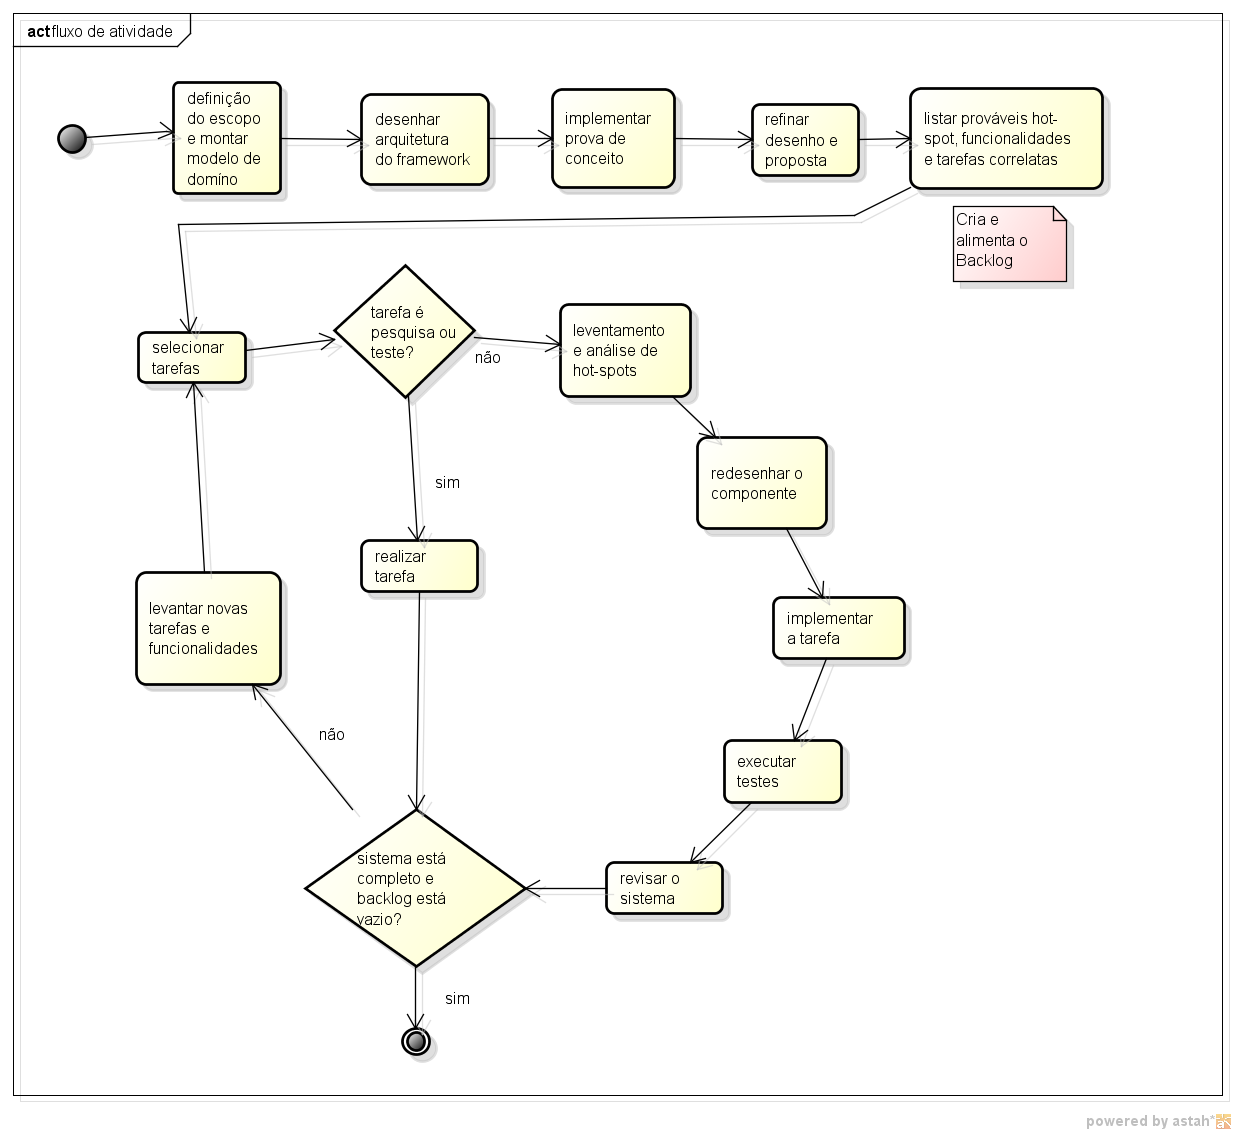
\includegraphics[keepaspectratio=true,scale=0.68]{figuras/fluxoatvd.png}
	\caption{fluxo de atividades propostas}
\end{figure}

As atividades iniciais compuseram a definição do tema, estudo do mesmo e execução da prova de conceito. Após seu refinamento foi criado o \textit{backlog} do sistema e o preencheu com todas as funcionalidades, \textit{hot-spots}, pesquisas e tarefas correlatas a serem realizadas. A partir de então iniciou-se as \textit{sprints}.

Cada \textit{sprint} possuiu as seguintes atividades que foram realizadas: 
\begin{itemize}
  \item Selecionar as tarefas a serem feitas nesta iteração;
  \item Caso a atividade seja apenas pesquisa ou teste no robô, é executada a tarefa e ao seu fim verificado se há mais tarefas no backlog para selecioná-las;
  \item Caso seja trabalho sobre o \textit{framework} é analisado se há algum \textit{hot-spot} nas funcionalidades selecionadas;
  \item Refinar o desenho do componente trabalhado caso necessário para receber a nova funcionalidade e o novo \textit{hot-spot} (se houver);
  \item Implementar a funcionalidade nova e rodar a suíte de testes;
  \item Fazer uma revisão de todo o sistema para ver se está evoluindo para o fim esperado e se há alguma falha arquitetural e,
  \item Verificar se ainda há trabalho a ser feito e, caso haja, levantar mais tarefas, testes e pesquisas para alcançar seu fim.
\end{itemize} 

\section{Resumo do Capítulo}

Para desenvolver o \textit{framework} foi usado o processo orientado a \textit{hot-spot} junto com a metodologias ágeis. A implementação foi dividida em iterações (\textit{sprints}) onde um \textit{hot-spot} e/ou funcionalidade era selecionada para ser realizado. Ele era então melhor analisado, estudado e projetado. Buscou-se que ao fim de cada \textit{sprint} uma nova funcionalidade ou \textit{hot-spot} tivesse sido desenvolvida e testada, além da arquitetura ser reavaliada para garantir que não houve depreciação da mesma com a implementação realizada.

A cada \textit{sprint} os \textit{hot-spots} foram avaliado para assegurar sua boa implementação e projeto e novas funcionalidades e \textit{hot-spots} levantados para alimentar o \textit{backlog}.